\documentclass[border=8pt]{standalone}

\usepackage{tikz}
\usetikzlibrary{arrows.meta, positioning, calc, backgrounds}
\usepackage{xcolor}
\usepackage{amssymb}

% Soft paper-friendly colors
\definecolor{rootfill}{HTML}{E3E4FA}
\definecolor{rootdraw}{HTML}{4B4E7A}

% Medium-soft lavender behavior colors
\definecolor{behAfill}{HTML}{F1EFF9}
\definecolor{behAdraw}{HTML}{635E84}

\definecolor{behBfill}{HTML}{E6E3F4}
\definecolor{behBdraw}{HTML}{5A547B}

\definecolor{behCfill}{HTML}{DAD4EE}
\definecolor{behCdraw}{HTML}{504875}

\definecolor{behDfill}{HTML}{CFC6E8}
\definecolor{behDdraw}{HTML}{463D6D}

% Medium-soft leaf/highlight colors
\definecolor{successfill}{HTML}{E0EEE4}
\definecolor{successdraw}{HTML}{55795B}
\definecolor{failfill}{HTML}{F1DBD8}
\definecolor{faildraw}{HTML}{8E5350}

\definecolor{goodpath}{HTML}{E0EEE4}
\definecolor{badpath}{HTML}{F1DBD8}

\begin{document}

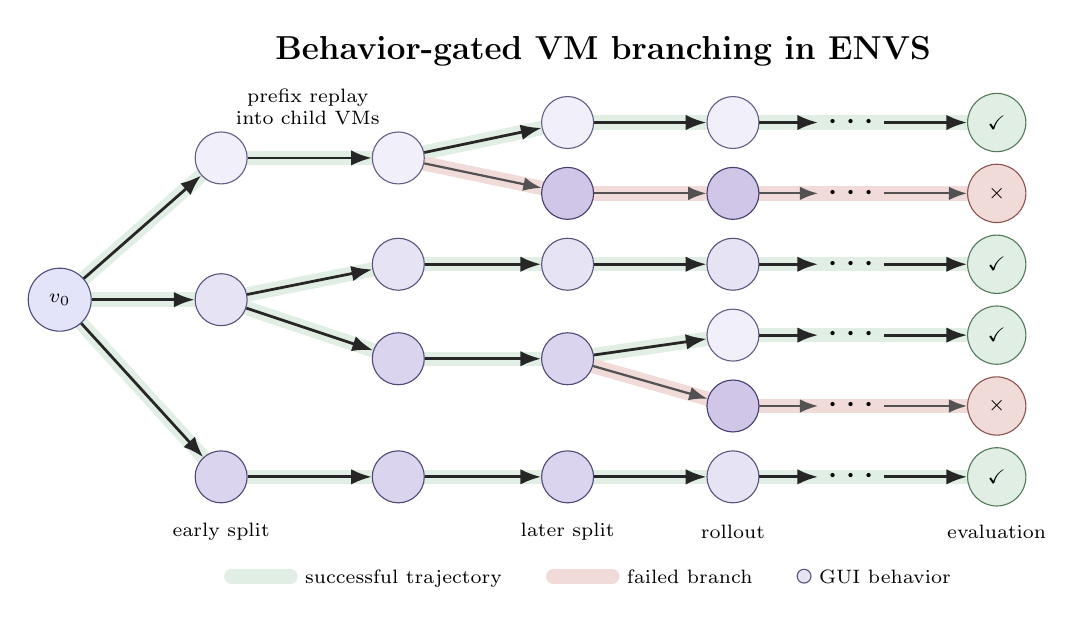
\begin{tikzpicture}[
    font=\small,
    >=Latex,
    x=1cm,
    y=1cm,
    state/.style={
        circle,
        draw=behAdraw,
        fill=behAfill,
        minimum size=6.6mm,
        inner sep=0pt
    },
    behA/.style={draw=behAdraw, fill=behAfill},
    behB/.style={draw=behBdraw, fill=behBfill},
    behC/.style={draw=behCdraw, fill=behCfill},
    behD/.style={draw=behDdraw, fill=behDfill},
    root/.style={
        circle,
        draw=rootdraw,
        fill=rootfill,
        minimum size=8.0mm,
        inner sep=0pt,
        font=\scriptsize
    },
    success/.style={
        circle,
        draw=successdraw,
        fill=successfill,
        minimum size=7.4mm,
        inner sep=0pt,
        font=\scriptsize
    },
    fail/.style={
        circle,
        draw=faildraw,
        fill=failfill,
        minimum size=7.4mm,
        inner sep=0pt,
        font=\scriptsize
    },
    edge/.style={->, line width=1.0pt, draw=black!85},
    thinEdge/.style={->, line width=0.8pt, draw=black!68},
    good/.style={line width=5.2pt, draw=goodpath, opacity=1.0, line cap=round},
    bad/.style={line width=5.2pt, draw=badpath, opacity=1.0, line cap=round},
    dots/.style={font=\Large},
    lab/.style={font=\scriptsize, align=center}
]

% ------------------------------------------------------------------
% Title
% ------------------------------------------------------------------
\node[font=\bfseries\large, align=center] at (6.9,3.15)
{Behavior-gated VM branching in ENVS};

% ------------------------------------------------------------------
% Highlighted trajectory segments
% Drawn on background layer so nodes/arrows stay in front.
% ------------------------------------------------------------------
\begin{scope}[on background layer]
    % Top retained path
    \draw[good] (0,0) -- (2.05,1.80);
    \draw[good] (2.05,1.80) -- (4.30,1.80);
    \draw[good] (4.30,1.80) -- (6.45,2.25);
    \draw[good] (6.45,2.25) -- (8.55,2.25);
    \draw[good] (8.55,2.25) -- (10.05,2.25);
    \draw[good] (10.05,2.25) -- (11.90,2.25);

    % Top failed branch
    \draw[bad] (4.30,1.80) -- (6.45,1.35);
    \draw[bad] (6.45,1.35) -- (8.55,1.35);
    \draw[bad] (8.55,1.35) -- (10.05,1.35);
    \draw[bad] (10.05,1.35) -- (11.90,1.35);

    % Middle retained path
    \draw[good] (0,0) -- (2.05,0.00);
    \draw[good] (2.05,0.00) -- (4.30,0.45);
    \draw[good] (4.30,0.45) -- (6.45,0.45);
    \draw[good] (6.45,0.45) -- (8.55,0.45);
    \draw[good] (8.55,0.45) -- (10.05,0.45);
    \draw[good] (10.05,0.45) -- (11.90,0.45);

    % Middle-lower retained path
    \draw[good] (2.05,0.00) -- (4.30,-0.75);
    \draw[good] (4.30,-0.75) -- (6.45,-0.75);
    \draw[good] (6.45,-0.75) -- (8.55,-0.45);
    \draw[good] (8.55,-0.45) -- (10.05,-0.45);
    \draw[good] (10.05,-0.45) -- (11.90,-0.45);

    % Middle-lower failed branch
    \draw[bad] (6.45,-0.75) -- (8.55,-1.35);
    \draw[bad] (8.55,-1.35) -- (10.05,-1.35);
    \draw[bad] (10.05,-1.35) -- (11.90,-1.35);

    % Bottom retained path
    \draw[good] (0,0) -- (2.05,-2.25);
    \draw[good] (2.05,-2.25) -- (4.30,-2.25);
    \draw[good] (4.30,-2.25) -- (6.45,-2.25);
    \draw[good] (6.45,-2.25) -- (8.55,-2.25);
    \draw[good] (8.55,-2.25) -- (10.05,-2.25);
    \draw[good] (10.05,-2.25) -- (11.90,-2.25);
\end{scope}

% ------------------------------------------------------------------
% Nodes
% Behavior colors encode executable GUI action fingerprints.
% At each branch point, child nodes use different shades.
% ------------------------------------------------------------------

% Root
\node[root] (r) at (0,0) {$v_0$};

% Top path
\node[state, behA] (a1) at (2.05,1.80) {};
\node[state, behA] (a2) at (4.30,1.80) {};

% a2 branches into different behaviors: a3=behA, af1=behD.
\node[state, behA] (a3) at (6.45,2.25) {};
\node[state, behA] (a4) at (8.55,2.25) {};
\node[dots]  (adots) at (10.05,2.25) {$\cdots$};
\node[success] (as) at (11.90,2.25) {$\checkmark$};

\node[state, behD] (af1) at (6.45,1.35) {};
\node[state, behD] (af2) at (8.55,1.35) {};
\node[dots]  (afdots) at (10.05,1.35) {$\cdots$};
\node[fail] (af) at (11.90,1.35) {$\times$};

% Middle path
\node[state, behB] (b1) at (2.05,0.00) {};

% b1 branches into different behaviors: b2=behB, c1=behC.
\node[state, behB] (b2) at (4.30,0.45) {};
\node[state, behB] (b3) at (6.45,0.45) {};
\node[state, behB] (b4) at (8.55,0.45) {};
\node[dots]  (bdots) at (10.05,0.45) {$\cdots$};
\node[success] (bs) at (11.90,0.45) {$\checkmark$};

\node[state, behC] (c1) at (4.30,-0.75) {};
\node[state, behC] (c2) at (6.45,-0.75) {};

% c2 branches into different behaviors: c3=behA, cf1=behD.
\node[state, behA] (c3) at (8.55,-0.45) {};
\node[dots]  (cdots) at (10.05,-0.45) {$\cdots$};
\node[success] (cs) at (11.90,-0.45) {$\checkmark$};

\node[state, behD] (cf1) at (8.55,-1.35) {};
\node[dots]  (cfdots) at (10.05,-1.35) {$\cdots$};
\node[fail] (cf) at (11.90,-1.35) {$\times$};

% Bottom path
\node[state, behC] (d1) at (2.05,-2.25) {};
\node[state, behC] (d2) at (4.30,-2.25) {};
\node[state, behC] (d3) at (6.45,-2.25) {};
\node[state, behB] (d4) at (8.55,-2.25) {};
\node[dots]  (ddots) at (10.05,-2.25) {$\cdots$};
\node[success] (ds) at (11.90,-2.25) {$\checkmark$};

% ------------------------------------------------------------------
% Arrows
% ------------------------------------------------------------------

% Root branches: branching edges may be diagonal
\draw[edge] (r) -- (a1);
\draw[edge] (r) -- (b1);
\draw[edge] (r) -- (d1);

% Top path
\draw[edge] (a1) -- (a2);
\draw[edge] (a2) -- (a3);
\draw[edge] (a3) -- (a4);
\draw[edge] (a4) -- (adots);
\draw[edge] (adots) -- (as);

% Top failed branch
\draw[thinEdge] (a2) -- (af1);
\draw[thinEdge] (af1) -- (af2);
\draw[thinEdge] (af2) -- (afdots);
\draw[thinEdge] (afdots) -- (af);

% Middle upper path
\draw[edge] (b1) -- (b2);
\draw[edge] (b2) -- (b3);
\draw[edge] (b3) -- (b4);
\draw[edge] (b4) -- (bdots);
\draw[edge] (bdots) -- (bs);

% Middle lower path
\draw[edge] (b1) -- (c1);
\draw[edge] (c1) -- (c2);
\draw[edge] (c2) -- (c3);
\draw[edge] (c3) -- (cdots);
\draw[edge] (cdots) -- (cs);

% Middle lower failed branch
\draw[thinEdge] (c2) -- (cf1);
\draw[thinEdge] (cf1) -- (cfdots);
\draw[thinEdge] (cfdots) -- (cf);

% Bottom path
\draw[edge] (d1) -- (d2);
\draw[edge] (d2) -- (d3);
\draw[edge] (d3) -- (d4);
\draw[edge] (d4) -- (ddots);
\draw[edge] (ddots) -- (ds);

% ------------------------------------------------------------------
% Labels
% ------------------------------------------------------------------

\node[lab, text width=2.0cm] at (3.15,2.45)
{prefix replay\\into child VMs};

\node[lab] at (2.05,-2.95) {early split};
\node[lab] at (6.45,-2.95) {later split};
\node[lab] at (8.55,-2.95) {rollout};
\node[lab] at (11.90,-2.95) {evaluation};

% ------------------------------------------------------------------
% Legend
% ------------------------------------------------------------------

\node[lab] at (6.75,-3.55) {
\begin{tabular}{@{}c@{\ }l@{\qquad}c@{\ }l@{\qquad}c@{\ }l@{}}
\tikz{\draw[good] (0,0) -- (0.75,0);} & successful trajectory &
\tikz{\draw[bad] (0,0) -- (0.75,0);} & failed branch &
\tikz{\node[state, behB, minimum size=5pt]{};} & GUI behavior
\end{tabular}
};

\end{tikzpicture}

\end{document}